\section{Experiment 2}
\subsection{Methodology} \label{method-2}

%<---------------------------->%
% Motivation
%% The second experiment takes a step futher
%%% First: Mimics an HCI setting (generalization)
%%% Second: Different perspective
%%% Third: Different impact setting
%% We created a HCI scenerio and measure participant's preference using Likert, QV and a monetary task.
%<---------------------------->%

The first experiment results demonstrated strong implication that QV aligns closer to the participant's real preference compared to the Likert scale when choosing among a spectrum of societal issues. To take a step further, we designed the second experiment with three changes compared to the previous experiment: 1) a change in topic domain, 2) a change in the relationship of items on the ballot, and 3) a change in the degree of the tangibility of the survey outcome. These three changes will allow us to understand QV's generalizability across different application scenarios. 

First, we changed the application domain form societal causes to an HCI application. Preference elicitation is a common theme in HCI studies. Unlike political and public-opinion surveys, HCI surveys often focus on users' preferences on designs and user experiences. Understanding user preferences is an essential step in creating and improving designs to fit the users' needs. 

Second, this experiment focused on items on the ballot that are of different \textit{perspectives} for the same subject matter, a common case in the HCI domain, rather than having different \textit{options} contributing to the same topic as we did in the first experiment. Recall we asked participants to choose among different societal causes (items) that impacted the society as a whole (topic). This subtle difference lies in the different \textit{relationships} between the items on the ballot. To give a simple analogy: if the first experiment asked about one's preference among chocolate, strawberry, and vanilla ice cream (options), the second experiment asked how much does one care about the texture, flavor, and color of ice cream (perspectives). 

Lastly, the second experiment focused on a setting that surveyed matters with a tangible and more immediate outcome to the participants compared to a more abstract and further-in-the-future impact. This difference  may impact the performance of QV and Likert.
% Many market research studies customer's experience with their product compared to governments that poll for people's opinions on mid to long term societal causes. 
% In experiment two, we changed the topic domain of the survey, elected different items to put on the ballot, and chose a more immediate-impact setting. 

We hypothesized that QV would still outperform Likert in accurately representing the participants' true preferences in the new setting. To test our hypothesis, we designed a between subject study with two groups of participants. Both groups of subjects participated in an HCI study using different surveying techniques, QV and Likert. In this section, we first explain how we decided on the HCI study scenario. Then, we demonstrate the experiment workflow accompanied by the interfaces of the experiment.

%<---------------------------->%
% HCI Experiment background
%% Video HCI experiments
%% Selection of the five elements and their definitions
%% The goal of this HCI experiment is to find elements that impact participants most.
%<---------------------------->%
 
\subsection{Choice of HCI study}
It is crucial for us to design an HCI study scenario that aligns with the three changes proposed in the previous subsection. We set out to find a typical use case where UX/UI researchers aim to prioritize features and elements that their users care about via surveys. On the one hand, we wanted to avoid creating an entirely new HCI study that required sophisticated verification. On the other hand, reproducing an HCI study that used Likert surveys can be costly and difficult because of the limited access to the devices, designs, or interfaces used in the study. Therefore, we concluded that we needed a new research question and study design involving surveys in a well-explored HCI topic to maintain ecological validity.

We created a video streaming experience HCI research scenario for this experiment. Research on video and audio elements of video playback from the lens of HCI has been relatively mature. Researchers provided insights to topics including multi-media conferencing \cite{watson1996evaluating}, video-audio perception \cite{chen2006cognitive, molnar2015assessing}, and, more specifically, trade-offs among various video and audio elements under network or monetary constraints \cite{molnar2013comedy, oeldorf2012bad}. \textcite{oeldorf2012bad}, for example, conducted a study to understand how users with bandwidth constraints made trade-offs covering a broad set of elements across multiple videos and audio elements. They examined participants' attitudes between three video bit rates, three video frame rates, and two audio sampling rates across three types of video content. Participants rated the overall quality, video quality, audio quality, and enjoyment level on a 5-point Likert scale in each condition. The study derived the conclusions from analyzing the means and standard deviations of the Likert survey results. This is a typical study to explore which one or some of the $K$ elements to prioritize under constraints.

We proposed a similar user research topic as that in \textcite{oeldorf2012bad}'s study and we designed the experiment to answer the following question: ``Given a video with unsatisfying quality, under limited bandwidth, how should the bandwidth be allocated to enhance the five video and audio elements, including stability of video imagery, stability of audio, quality of audio, quality of video imagery, and audio-video synchronization, to obtain a relatively satisfying video streaming experience from the viewers' perspective?'' We elected the five video playback elements based on the related work and defined them as the following: 

\begin{itemize}
    \item Motion Smoothness (Stability of Video Imagery) \cite{claypool1999effects}: Motion smoothness refers to how smoothly the visuals of the video plays. Lost video packets during playback due to limited bandwidth causes froze frames and undermines the stability of the video imagery. The higher the  video packets lost percentage is, the more staggered the video seems.
    \item Audio Stability \cite{claypool1999effects}: Audio stability refers to how smoothly the audio of the video plays. Lost audio packets during playback due to limited bandwidth creates silence and undermines the stability of the audio. The higher the audio packets lost percentage is, the more stuttered the audio sounds.
    \item Video Resolution (Quality of Video Imagery) \cite{oeldorf2012bad, knoche2008low}: Video resolution refers to how sharp the visuals in the video looks. With a lower resolution, i.e., lower pixel density per inch, the video imagery is pixelated and unclear. At the same time, a playback with a lower video resolution may be a fallback option under limited bandwidth since it requires a smaller video file.
    \item Audio Quality \cite{oeldorf2012bad, noll1993wideband}: Audio quality refers to how clear and crisp the sound quality is of the video. With a lower audio sampling rate, the audio sounds more muffled and unclear. At the same time, a playback with a lower audio quality would be a fallback option under limited bandwidth since it requires a smaller audio file.
    \item Audio-Video Synchronization \cite{steinmetz1996human}: ``Audio-video Synchronization'' represents how well video visuals synchronized with the audio playback. In our experiment, we focused only on the type of asynchronization where the audio plays ahead of the video. Under bandwidth constraint, visuals and audio may be out of sync due to the insufficient bandwidth to transmit both of them promptly at the same time.
\end{itemize}

No previous studies have looked at the combination of all five video and audio elements at once, but some have studied one or a few of them together. Hence, this is a valid HCI-related research question. 
% we make use of individual studies to decide the value associated with the different levels of changes for each of these elements. 
In the next section, we describe our video-audio experiment that aims to compare the performance between Likert and QV surveys in their ability to answer the research question in identifying the video/audio elements that impact participants' streaming experience the most.

% We might need a paragraph on what kind of video we use and why we use that video. Here is a snippet of text to use.
% In this experiment, we clipped a 90-second weather forecast video for the United States. There are several reasons why we choose the weather forecast. First of all, the concept of a weather forecast is generic and universal. The terms used in the weather forecast can be considered common knowledge. Video clips such as sports can contain specific jargon while move clips can be unfamiliar to some and not to others. Second, since we are altering both audio and video, we wanted a video that contained a large amount of visualization but also provided information through speech. Drama and talk shows, for example, would lean towards visual elements or audio elements. Finally, visual and audio elements in a weather forecast complement each other. The meteorologist usually spoke aloud the weather with visual cues such as an icon.


\begin{figure}[htpb]
    \centering
    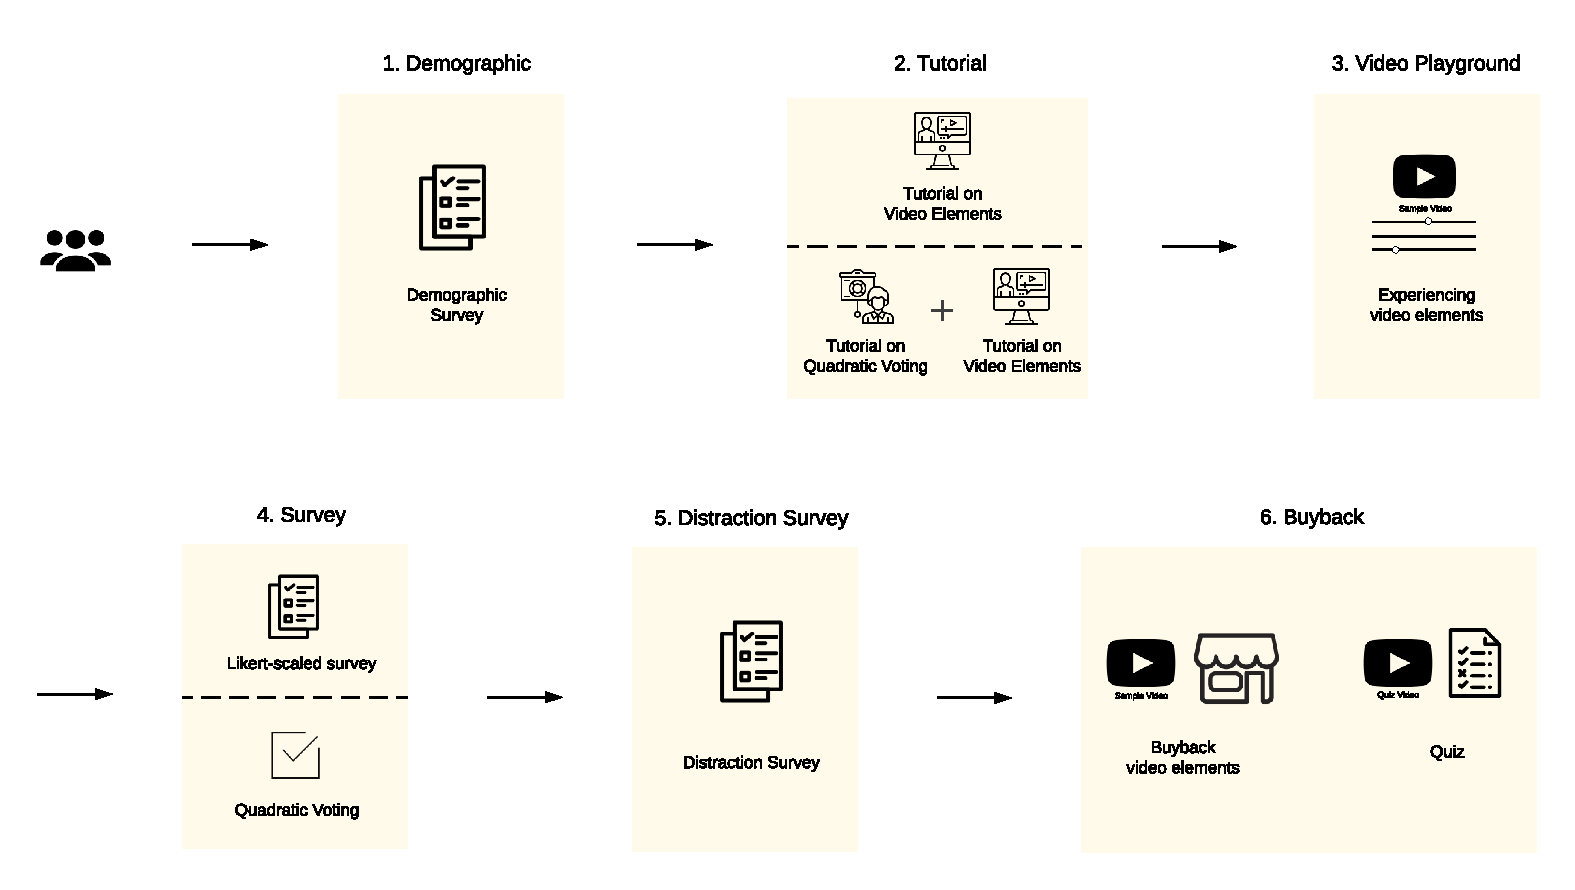
\includegraphics[width=\textwidth, keepaspectratio=true]{content/image/new_exp2_flow.pdf}
    \caption{
        Experiment two is conducted between subjects. There are two groups of participants. Steps with dashed lines indicated difference among the two groups. The one on top is for the Likert group while the one on the bottom is for the QV group. Participants would go through six steps in total.
    }
    \label{fig:exp2_flow}
\end{figure}

\subsection{Experiment Flow}

% We recruited 180 participants through MTurk. 
To compare how well Likert survey and QV reflect people's underlying preferences, we designed the following experiment. We recruited participants through MTurk. We divided participants equally into two groups: Likert and QV. All participants followed six steps, each represented in a shaded area in Figure \ref{fig:exp2_flow}. The six steps are: (1) demographics survey, (2) tutorials and attention checks, (3) a video playground, (4) a Likert or QV survey to express preferences, (5) a distraction survey, and (6) the buyback task. Now we explain the five steps in detail.

\subsubsection{Step 1. Demographic}
We greeted participants with a consent form. In the consent form, we told the participants that we wanted to collect people's thoughts across different video playback elements. We did not reveal to the participants that this experiment aims to compare Likert and QV until the participants completed the experiment. Once participants gave their consent, participants would fill out a demographic survey. The demographic survey is identical to the first experiment.

\subsubsection{Step 2. Tutorials and attention checks}
In the second step, we provided both groups of participants context and background information of the experiment. For both groups, we asked them to complete a tutorial on the definition of the five different video and audio elements of video-playback, as described in the previous subsection. In the tutorial, for each element, we showed a pair of videos side-by-side to compare how the same video would differ if a particular element was at the worst quality in the range we studied compared to when it was at the best quality in our range, keeping the other four elements the same at their best quality. The participants are required to start playing each Once the participants thought they understood the concepts, we asked them to answer five multiple choice questions related to the concepts in the tutorial. Participants that failed to answer four out of five questions correctly were disqualified from completing the remaining experiment. This assured that participants fully understood the terminology used in the experiment and were taking the experiment seriously. 

For the QV group, given that QV is unpopular among the mass, we added an additional tutorial on QV and attention checks specific to QV prior to the video element tutorial. This tutorial is similar to the one in experiment one where we provided a QV video tutorial and a QV playground for participants to play with. The quiz consists of five true false questions. Participants that answered two or more incorrectly will be disqualified.

\begin{figure}[htpb]
    \centering
    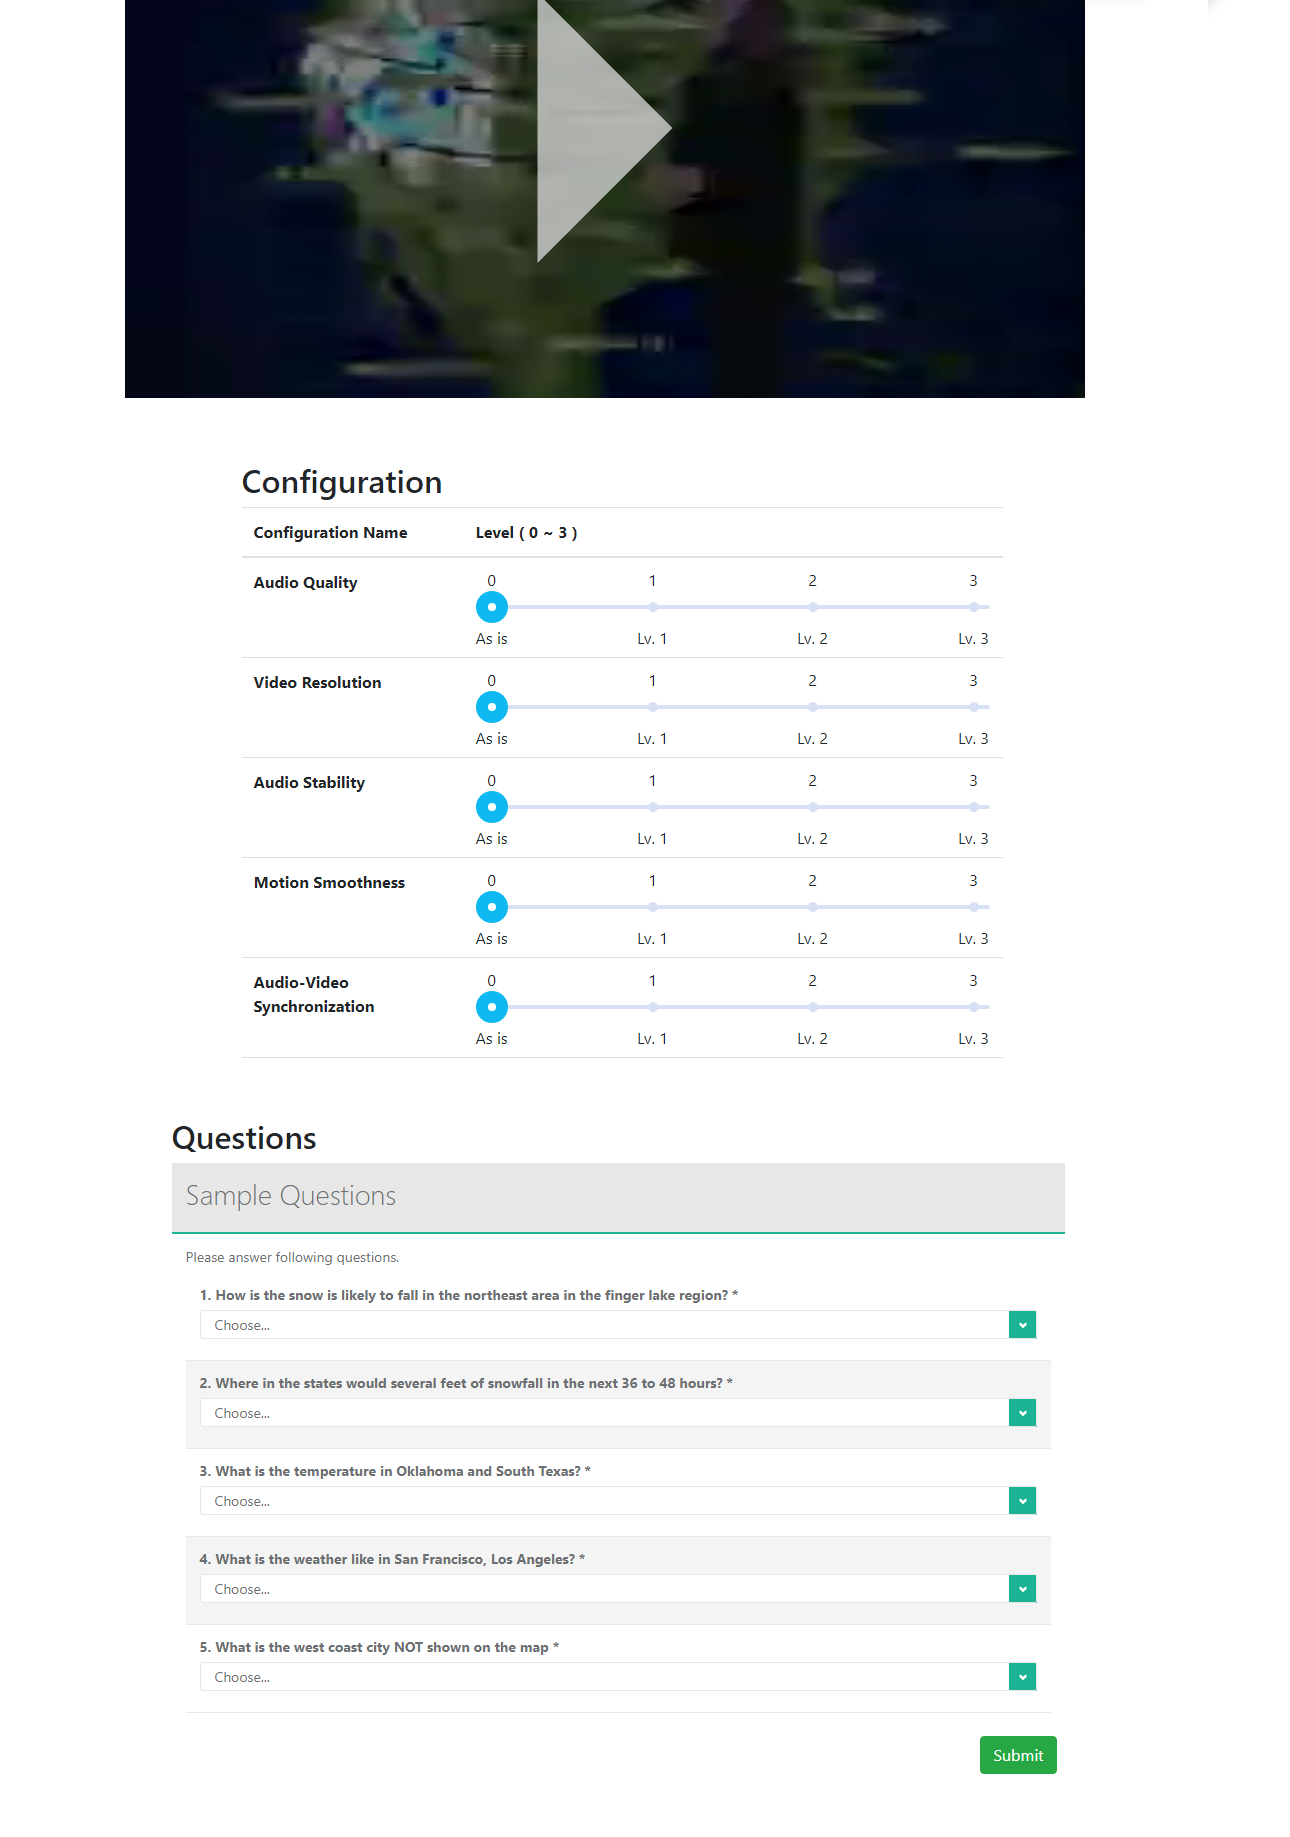
\includegraphics[width=\textwidth, keepaspectratio=true]{content/image/exp2_playground.png}
    \caption{
        The Real-time Video Element Interface allows participants to adjust and understand how different levels of video playback element impacts their viewing experience. Participants were asked to complete the five multiple choice questions relevant to the video content.
    }
    \label{fig:exp2_playground}
\end{figure}


\subsubsection{Step 3. Video Playground}
Once participants passed the attention checks, we reminded them that our goal was to implement a video streaming service on international flights with limited bandwidth. We first showed them the current prototype of streaming service under limited bandwidth, which was a weather forecast video with all five elements at the worst quality in the range we designed to study\footnote{Motion smoothness: 32\% packet loss rate; Audio stability: 32\% packet loss rate; Video resolution: 210x280; Audio quality: 8kHz sampling rate; Audio-video synchronization: audio plays 2250ms ahead of the video}. After experiencing the current prototype, the participants moved on to the next page.

We then instructed them to explore how various levels of enhancement on different elements in the current prototype would improve the viewing experience. To help them better understand the impact of the enhancements, we built a video playground shown in Fig \ref{fig:exp2_playground}. This playground showed real-time changes in the overall quality of the video as the participants adjust the control panel to a specific combination of different levels of enhancements for the five video elements.

This interface showcased a weather forecast video on the top of the page. For each of the five video playback elements, we provided a slider with four levels of tickers. Participants can toggle any of these five elements to any of the five levels at any time. According to the quality levels the participants set, the video playback will immediately apply those changes. Participants can pause and play the video at any time, and they can replay the video as many times as they like. We encouraged participants to test out different combinations freely in this playground.

The five levels for each element covered the full range of quality we wished to explore in the experiment, with Level 0 at the lowest quality and Level 4 at the highest. We designed the intermediate levels based on prior research \cite{claypool1999effects,oeldorf2012bad, noll1993wideband,knoche2008low, steinmetz1996human} such that the changes between each level of an element have a quasi-linear impact on viewers' perception. The five levels of the five video playback elements are listed below, from Level 0 to Level 4:
\begin{itemize}
    %20\%, 8\%, 4\%, and 0\%
    \item Motion Smoothness: 32\%, 20\%, 8\%, 4\%, and 0\%
    %20\%, 8\%, 4\%, and 0\%
    \item Audio Stability: 32\%, 20\%, 8\%, 4\%, and 0\%
    %210x280, 294x392, 364x486, and 420x560     
    \item Video Resolution: 210x280, 294x392, 364x486, 420x560, and 600x800 
    %8kHz, 11kHz, 16kHz, and 48kHz 
    \item Audio Quality: 8kHz, 11kHz, 16kHz, 48kHz, and 96kHz
    %1850, 1615, 1050, or 0 ms ahead
    \item Audio-Video Synchronization: 2250ms, 1850ms,  1615ms, 1050ms, or 0ms ahead
\end{itemize}

In addition to the control panel, we added five multiple-choice questions at the bottom of the same page. These questions asked factual questions based on the content of the weather forecast video. We told participants that their responses would be invalidated if they answer three or more multiple-choice questions incorrectly. These questions made sure that participants finished watching the video at least once. Further, these questions ensured that all the participants were on the same page that the goal of video streaming in our experiment was primarily to understand the content of the video, and not for pure entertainment purposes.

\subsubsection{Step 4. Surveying Preferences}
After the participants were confident that they understood how the enhancements on different video playback elements would impact their viewing experience and answered the five multiple-choice questions, we surveyed the participants about their feedback on how critical the enhancements for the current prototype on each of the five video elements were for the purpose of understanding the content of a weather forecast video. The Likert Group responded with a five-point Likert scale survey. The QV group used the QV interface similar to that of the first experiment. The only difference compared with Figure \ref{fig:qv_donation} is that instead of societal causes, we list the five video elements as options. According to our findings from experiment 1, we designed the credit budget to be 100 voice credits, derived from $N^2 x O$, where $N=5$ and $O=4$.


\subsubsection{Step 5. Distraction Survey}
After the surveys in step 4, the remaining steps of the experiment aimed to collect participants' ground-truth preference on the same question asked in the survey. 
% Since we compared QV and Likert responses to the ground-truth preference to evaluate how aligned they were, we would like to keep the responses in the survey independent from the ground-truth preference collected via the buyback task. 
To ensure the accuracy of the ground-truth preference, similar to experiment one, we wanted to prevent participants from translating their survey results directly to the buyback task in the next step without careful deliberation on the buyback. Therefore, we designed a distraction survey after the Likert or QV survey and before the buyback task. The survey asked about the participants' preferences on what type of content they would like to stream in flight.


\subsubsection{Step 6. Buyback}
Participants completed the experiment with a \textbf{buyback task}. The goal of this task is to capture a participant's actual underlying preferences on the same question asked in the survey: how critical the enhancements for the current prototype on each of the five elements were for understanding the content of a weather forecast video. 
% It is non-trivial, compared to the previous experiment's donation task, to measure one's real preference across different video playback elements. We designed \textbf{the buyback task} to capture this preference. Participants were told about the possibility of earning a bonus during this task.

Participants were now given the same weather forecast video served via the current prototype under limited internet bandwidth. We provided the participants a budget of \$40 to shop in a ``video element store.'' The store allowed participants to purchase enhancements for the five video elements, as presented in Figure \ref{fig:exp2_store}. We told the participants that they could ``enhance'' each of these elements by``spending'' on each of them. The more they spent on an element, the more enhancement they would see for the element. 
% because they will use the combination they purchased to complete the next task. 

Participants were aware that they would next need to answer a quiz with five factual questions on a different weather forecast video that was enhanced based on their current purchase. We also listed some example questions on the same page as the buyback store to assist participants in making their purchase decisions. Only if a participant answered four out of five multiple-choice questions correctly, would they qualify for a lottery that paid the winners their remaining amount in the \$40 budget after their purchase. For example, if the winning participant spent 30 dollars and answered four out of the five questions correctly, they would win 10 dollars because their total budget is 40 dollars. 

This provides an incentive-compatible setting to the participants. Participants, assuming being rational, would find a balance for each of the elements based on their willingness to pay (WTP). To gain the maximum return, participants would purchase the minimum required enhancement they needed to complete the quiz for each elements. Any additional purchase would decrease their reward in the lottery. Any less purchase would hurt their chance of being qualified for the lottery.
% This setting is somewhat common in real life, where many subscription-based services on the market require customers to pay additional premiums for additional benefits. Another example is gamers making purchases in stores that equip online avatars with extra features to compete with other players in online games. We believe that with tasks in hand, participants will consider the best use of their budget and understand the content in the video. The Quiz ensures that participants have correctly comprehended the video.

\begin{figure}[htpb]
    \centering
    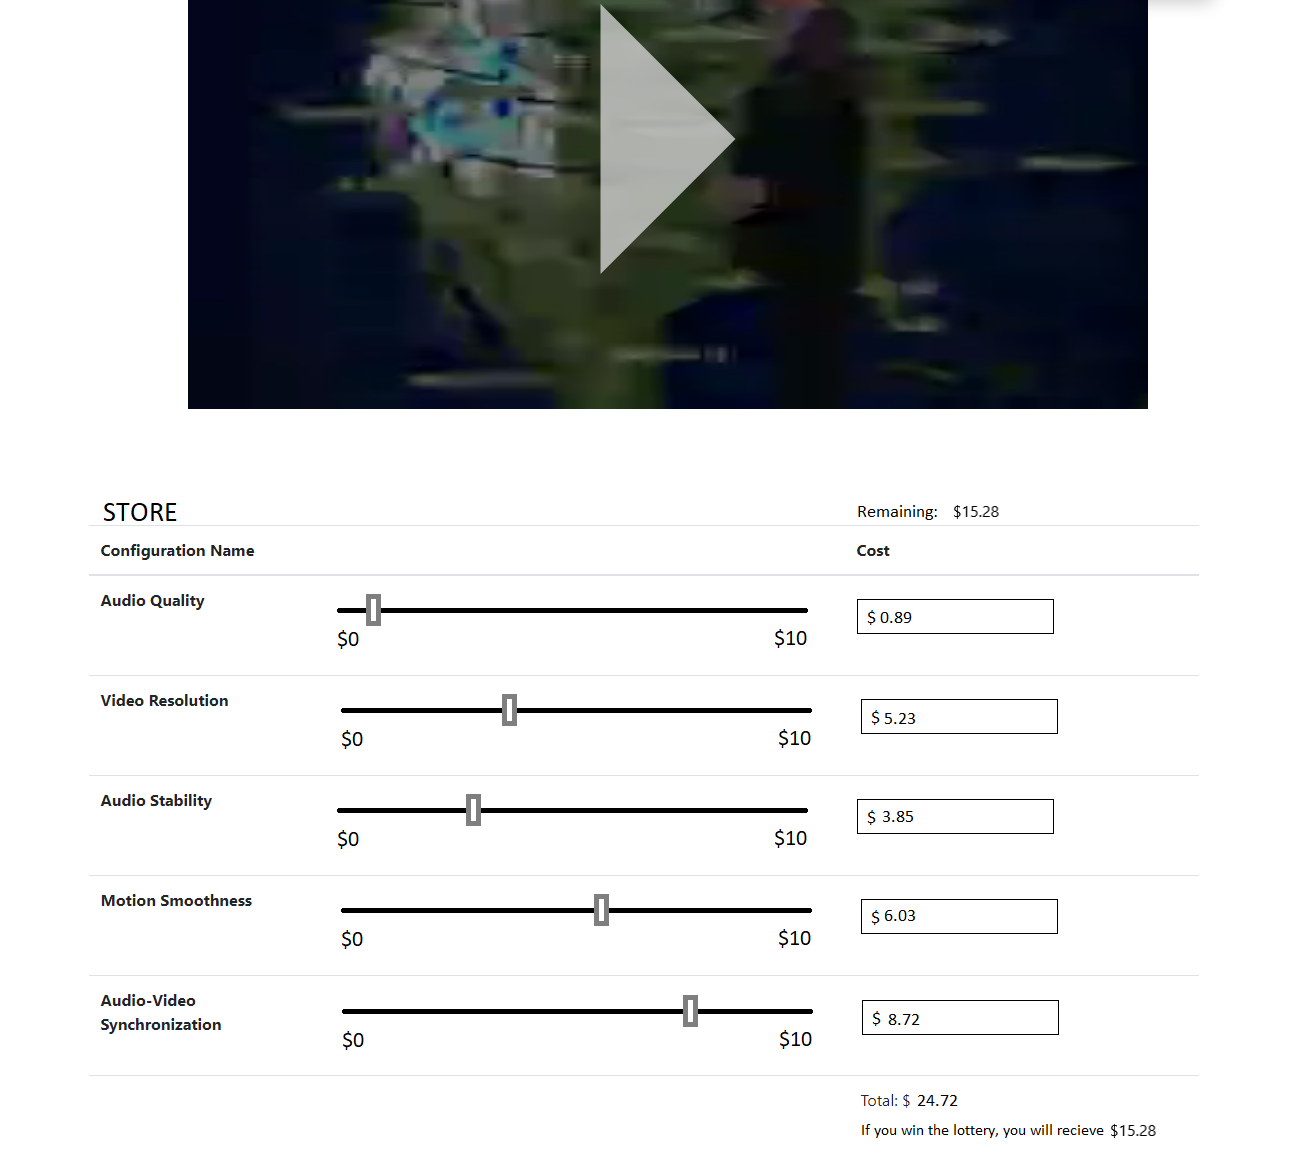
\includegraphics[width=\textwidth, keepaspectratio=true]{content/image/bb_store.png}
    \caption{
        Interface of the buyback store. This store allows participants to enter any amount they want to spend for a particular item. The interface maps the monetary input to a predefined level of enhancement and renders the change in the video in real-time.
    }
    \label{fig:exp2_store}
\end{figure}

Notice that different from the playground, the store provides a continuous slider that can stop at any location along the line instead of tickers at discrete levels for the participants to input a monetary amount. Each slider is accompanied by a text input box to the right. Participants can stop the slider anywhere, and the system would map the slider's relative position to a dollar amount between \$0 and \$10, representing the dollar amount spent on enhancing an element. Alternatively, participants can enter a dollar value between \$0 and \$10, and the slider would move to the corresponding location.

In the system back-end, each monetary value $M_i$ maps to one of the nine enhancement levels. The nine enhancement levels cover the same range we presented in the video playground with more granular quasi-linear divisions. This means that we are not altering participants' previous experience, but allowing them to experience and purchase more fine-grain enhancements. Since \$10 is linearly mapped to nine levels, where Level 0 is worth \$0, $M_i$ translates to Level $roundup(M_i/1.25)$. For example, spending \$4.2 on an element will enhance that element to Level 4. When the slider moves, the video above reflects the change in enhancement level immediately. The nine enhancement levels for the five elements and the corresponding costs are shown in~\Cref{nine-level-data}.

However, participants were not aware of \textbf{how many} levels exist in this control panel and \textbf{where} the cutoffs are. One consideration is that by hiding the number of levels present, participants now have the freedom to put in any value that they ``believe'' they want to devote. The ``ticks'' do not constrain participants we presented since they do not know \textit{where} each level changes, making their input value truthful.
% The interface will automatically translate the input value (between 0 and 10) into nine different levels. The mapping between the cost is the cost divided by 1.25. This is because there are a total of eight enhancement levels. In the case of the image, Audio Quality will be mapped to Level 0, and Video Resolution will be mapped to Level 4 and so on.

% We list the nine levels here:
% \begin{itemize}
%     %20\%, 8\%, 4\%, and 0\%
%     \item Stability of Video Imagery: 30\%, 25\%, 20\%, 12\%, 8\%, 6\%, 4\%, 2\%, and 0\%
    
%     %20\%, 8\%, 4\%, and 0\%
%     \item Stability of Audio: 30\%, 25\%, 20\%, 12\%, 8\%, 6\%, 4\%, 2\%, and 0\%
    
%     %8kHz, 11kHz, 16kHz, and 48kHz 
%     \item Quality of audio: 8kHz, 9.5kHz, 11kHz, 13kHz, 16kHz, 32kHz, 48kHz, 64khz, and 96kHz
    
%     %210x280, 294x392, 364x486, and 420x560     
%     \item Quality of the video: 160x214, 180x240, 210x280, 240x320, 294x392, 320x427, 364x486, 390x520, and 420x560 
    
%     %1850, 1615, 1050, or 0 ms ahead
%     \item Audio-Video Synchronization: 2400, 2100, 1850, 1700, 1615, 1300, 1050, 500ms or 0 ms ahead
% \end{itemize}


\begin{table}[]
\footnotesize
\centering
\begin{tabular}{|c|c|c|c|c|c|c|c|c|c|}
\hline
\textbf{\begin{tabular}[c]{@{}c@{}}Playground\\ Level\end{tabular}} & \textbf{0} & \textbf{} & \textbf{1} & \textbf{} & \textbf{2} & \textbf{} & \textbf{3} & \textbf{} & \textbf{4} \\ \hline
\textbf{\begin{tabular}[c]{@{}c@{}}Buyback\\ Enhancement \\ Level\end{tabular}} & \textbf{\$0} & \textbf{\begin{tabular}[c]{@{}c@{}}(\$0, \\ \$1.25{]}\end{tabular}} & \textbf{\begin{tabular}[c]{@{}c@{}}(\$1.25,  \\ \$2.5{]}\end{tabular}} & \textbf{\begin{tabular}[c]{@{}c@{}}(\$2.5, \\ \$3.75{]}\end{tabular}} & \textbf{\begin{tabular}[c]{@{}c@{}}(\$3.75, \\ \$5{]}\end{tabular}} & \textbf{\begin{tabular}[c]{@{}c@{}}(\$5, \\ \$6.25{]}\end{tabular}} & \textbf{\begin{tabular}[c]{@{}c@{}}(\$6.25, \\ \$7.5{]}\end{tabular}} & \textbf{\begin{tabular}[c]{@{}c@{}}(\$7.5, \\ \$8.75{]}\end{tabular}} & \textbf{\begin{tabular}[c]{@{}c@{}}(\$8.75, \\ \$10{]}\end{tabular}} \\ \hline
\textbf{\begin{tabular}[c]{@{}c@{}}audio\\ quality (kHz)\end{tabular}} & 8 & 9 & 11 & 13 & 16 & 32 & 48 & 72 & 96 \\ \hline
\textbf{\begin{tabular}[c]{@{}c@{}}video\\ resolution\end{tabular}} & 210x280 & 249x332 & 294x392 & 327x436 & 364x486 & 390x520 & 420x560 & 480x640 & 600x800 \\ \hline
\textbf{\begin{tabular}[c]{@{}c@{}}audio\\ loss   (\%)\end{tabular}} & 32 & 26 & 20 & 14 & 8 & 6 & 4 & 2 & 0 \\ \hline
\textbf{\begin{tabular}[c]{@{}c@{}}video\\ loss (\%)\end{tabular}} & 32 & 26 & 20 & 14 & 8 & 6 & 4 & 2 & 0 \\ \hline
\textbf{\begin{tabular}[c]{@{}c@{}}audio\_video\\ sync (ms)\end{tabular}} & 2250 & 2000 & 1850 & 1750 & 1615 & 1375 & 1050 & 825 & 0 \\ \hline
\end{tabular}
\caption{Mapping of Levels and Costs in Buyback. The first column outlines the variables used for different levels in the video-streaming playground. The second column maps the buyback cost to each configuration. Do note that participants do not know how the monetary maps to the configurations.}
\label{nine-level-data}
\end{table}



% There are several considerations for this design. One consideration is that by hiding the number of levels present, participants now have the freedom to put in any value that they ``believe'' they want to devote. The ``ticks'' do not constrain participants we presented since they do not know \textit{where} each level changes, making their input value truthful. Another consideration is that the nine levels cover the same range as the four levels presented in the video playground. This means that we are not altering participants' previous experience, but allow them to experience and purchase more fine-grain enhancements. 
We chose the budget and the monetary costs of these levels based on a pilot experiment to ensure that participants can accomplish the tasks without spending all their budgets. We detail this pilot and the choice of budget in the appendix.

Once the participant made the purchase, they would see a new weather forecast video. This time the levels of enhancement is fixed with what the participants purchased. On this page, participants can replay the video as many times as they want and answer the five factual multiple-choice questions on the same page. This means participants do not need to memorize the content of the video. We ask participants questions like "What is the weather of Chicago?", "What is the highs and lows of San Diego," and "Which city was not shown in the video?". 
% These questions are similar to the ones we presented in the video playground. 
We also listed some example questions on the same page as the buyback store to assist participants in making their purchase decisions. 

\subsection{System Design}
In this experiment, we build on top of the system for experiment one. To create real-time adjustments, we created the different qualities of video and audio files independently ahead of the experiment. When there is a change in the audio or video quality toggle, the system serves the correct combinations of video and audio files. JavaScript in the front-end was responsible for creating the video-audio synchronization and video/audio packet loss effects.
This design balances the need for network speed, preventing from streaming every configuration from the server. It also prevents the need for a powerful client such that video and audio qualities were not computed directly on the client. The experiment source code for experiment two is publicly available \footnote{Not yet public}, and so is the video interface as a stand-alone repository \footnote{https://github.com/hank0982/QV-app}.